\documentclass[11pt]{article}
\usepackage[margin=1in]{geometry}
\usepackage[T1]{fontenc}
\usepackage[utf8]{inputenc}
\usepackage{lmodern,microtype,amsmath,amssymb,graphicx,booktabs,longtable,tabularx,array}
\usepackage[round,authoryear]{natbib}
\usepackage{caption,subcaption,placeins,needspace}
\usepackage[hidelinks]{hyperref}
\hypersetup{pdftitle={Evolution and Reinforcement Learning in Changing Environments},pdfauthor={Abhinav Guntaka},pdfsubject={Research manuscript}}
\usepackage{enumitem}
\setlist{nosep}
\captionsetup{font=small,labelfont=bf}
\setlength{\parskip}{0.25em}
\setlength{\emergencystretch}{2em}
\widowpenalty=10000
\clubpenalty=10000
\renewcommand{\arraystretch}{1.12}
\newcolumntype{Y}{>{\raggedright\arraybackslash}X}
\newcolumntype{P}[1]{>{\raggedright\arraybackslash}p{#1}}
\newcommand{\IQM}{\operatorname{IQM}}
\newcommand{\E}{\mathbb{E}}
\title{Evolution and Reinforcement Learning\\in Changing Environments}
\author{Abhinav Guntaka}
\date{}
\begin{document}
\maketitle
\vspace{-2em}
\begin{abstract}
We compare ecological neuroevolution (OE), evolution strategies (ES) and proximal policy optimization (PPO) in a simulated foraging world. Six separately tuned fixed- and varied-environment configurations train for the same nominal agent-step budget, with ten runs each. We measure food acquisition before and during adaptation to thirty test environments and population persistence without replacement support. Across twenty shifted environments, OE performs below PPO with domain randomization (PPO-DR): the difference in interquartile mean of normalized adaptation area under the curve is $-0.5592$ (nominal 95\% bootstrap interval $[-0.6088,-0.5196]$). Varied OE also performs below OE-fixed. ES-DR slightly exceeds ES-fixed, whereas PPO-DR's small advantage over PPO-fixed is nonsignificant in the prespecified rank test. OE has poorer population persistence than PPO-DR and depends heavily on its population floor: externally supplied replacements account for over 99\% of births during resource-scarce adaptation.
\end{abstract}
\section{Introduction}
\citet{milano2019moderate} found that environmental variation across generations improved evolved controllers, with the best performance at a moderate rate of change. Ecological neuroevolution imposes a different selection pressure: agents must acquire enough food to survive and reproduce. Food acquisition also determines task performance, but selection through survival may favor different controllers from direct optimization of food intake.

We compare ecological neuroevolution (OE), evolution strategies (ES) and proximal policy optimization (PPO) in a continuous two-dimensional foraging world. OE maintains an interacting population with energy-dependent death and reproduction, supplemented by a minimum population of externally supplied replacements. ES and PPO optimize food acquisition and deploy copies of a single controller. Each method has separately tuned fixed- and varied-environment configurations. We evaluate food acquisition before and during adaptation, then measure population persistence in a separate assay without replacements.

A supporting experiment with inherited traits and fixed behavioral rules examines search objectives, mutation and cloning (Appendix~\ref{app:trait}).

We predicted that varied-environment OE would outperform PPO with domain randomization during adaptation. OE instead starts below PPO-DR and remains below it throughout the measured interval. Varied OE also scores below fixed OE; a later ES comparison favors the varied configuration by a smaller amount.

\section{Related work}
\citet{milano2019moderate} varied the rate of environmental change during evolution. \citet{milano2024qualitative} compared ES and PPO across tasks and treatments of environmental variation. Our experiment compares separately selected fixed- and varied-training configurations in a foraging task without sweeping the rate of environmental change.

\citet{hamon2023eco} studied persistent neural-agent populations with physiology-dependent reproduction and death. \citet{nisioti2022plasticity} used a minimal ecological model and ablations to distinguish fitness-based selection from niche-limited competition. Our implementation also couples survival and reproduction to agent behavior, but uses feedforward controllers and externally supplied population replacements.

Prior comparisons examine curricula \citep{nisioti2025transfer}, sequential changes and forgetting \citep{nisioti2026continual}, and update and inheritance regimes in ecological evaluations \citep{ge2026arena}. Here, adaptation begins independently from the trained snapshot in each test environment and permits further parameter updates.


\section{Experimental design}
\label{sec:methods}
\subsection{Foraging environment and controllers}
Agents move in a square arena with walls and regenerating food. Their observations contain 30 values: eight directional sectors for each of food, other agents and walls; current energy; the previous two-dimensional action; and three body traits. A feedforward controller has two hidden layers of 32 tanh units and two outputs, controlling turn and forward speed. Every method uses this actor architecture. Maximum speed, size and sensing range are fixed at 1, 1 and 10, respectively. 

Energy decreases with time, movement and sensing. A food item supplies 40 energy units; an agent starts with 100 and dies when its energy reaches zero. In ecological mode, agents can reproduce above an energy threshold, paying an energy cost for each offspring; they also die at a maximum age. Appendix~\ref{app:implementation} gives the full settings. Episodic competence evaluation uses the same movement, sensing and food dynamics, without reproduction.

Varied training samples arena size, food supply, layout and regrowth from the ranges in Table~\ref{tab:env}. The fixed environment has side length 60, 40 food items, a uniform layout and regrowth probability 0.03. Validation uses 20 sampled training-range environments and four corner cases. We fix thirty test environments before final evaluation: ten within the training ranges (T1), ten smaller, resource-scarce environments with clustered food (T2), and ten with food drift and seasonal relocation (T3). T3 retains the training ranges for the remaining parameters.

\begin{table}[tb]
\centering\small
\caption{Training and fixed test suites. Each test suite contains ten environments. The canonical fixed-training setting is given in the text. Unused layout parameters have no effect in a given environment.}\label{tab:env}
\begin{tabularx}{\linewidth}{lYYY}
\toprule
Parameter & Varied training / T1 & T2 & T3\\\midrule
Arena side $L$ & 40--80 & 30--40 & 40--80\\
Food items $F$ & 20--60 & 10--20 & 20--60\\
Layouts & Uniform, clusters, patches & Clusters & Uniform, clusters, patches\\
Cluster count $k$ & 2--5 & 2--3 & 2--5\\
Cluster scale $\sigma$ & 3--8 & 2--4 & 3--8\\
Patch radius & 4--10 & Not used & 4--10\\
Regrowth probability & 0.01--0.05 & 0.005--0.01 & 0.01--0.05\\
Food drift & 0 & 0 & 0.05--0.3\\
Season period (steps) & None & None & 100--300\\
\bottomrule
\end{tabularx}
\end{table}


\subsection{Training procedures}
\label{sec:procedures}
\paragraph{Ecological neuroevolution.}
OE starts with 32 agents and permits at most 128. Each agent has its own controller, and offspring inherit the parent's weights with Gaussian perturbations. In varied OE, the environmental parameters change every 2,000 world steps while the population continues. OE-fixed retains the canonical environment. During adaptation, either variant continues evolving in the assigned test environment.

Both variants maintain a population floor of 16. After a step below that floor, missing agents are replaced with mutated offspring of uniformly sampled surviving, non-newborn agents; if none are available, agents alive at the start of the step supply the parents. Replacements receive birth energy and a new position. We count natural and floor births separately.

\paragraph{Evolution strategies.}
ES optimizes the shared actor weights using \texttt{Open\_ES} in evosax \citep{salimans2017evolution,lange2023evosax}, with antithetic perturbations and centered-rank fitness shaping. ES-DR samples training environments; ES-fixed uses the canonical environment. Evaluation uses the strategy mean.

Each candidate is evaluated with 16 policy copies in 500-step worlds without births. Its score is food per initial agent, averaged over its configured episodes. Candidates in a generation share environment draws and reset/step random keys; ES-DR redraws the episode environments each generation.

\paragraph{Proximal policy optimization.}
PPO uses a clipped policy-gradient objective \citep{schulman2017proximal}, a separate value network, and a shared policy across agents in 64 parallel episodic worlds. Food acquisition supplies the reward. PPO-DR samples environment parameters at episode resets; PPO-fixed uses the canonical environment. Training actions are stochastic; competence evaluation uses deterministic actions. We adapt PureJaxRL's continuous-action PPO (Appendix~\ref{app:implementation}).

Each world contains 16 agents and restarts at 500 steps or when all agents die. An agent's death terminates its trajectory. Steps beginning with a dead agent are excluded from losses and advantage normalization; when enabled, reward-normalization statistics are collected over living agents.

Table~\ref{tab:procedures} summarizes deployment and transfer.

\begin{table}[tb]
\centering\small
\caption{Training and transfer procedures. Each row has fixed and varied variants, separately tuned. Body traits and actor architecture are shared.}\label{tab:procedures}
\begin{tabularx}{\linewidth}{lYYY}
\toprule
Procedure & Training signal & Competence deployment & State at adaptation start\\\midrule
OE & Energy-dependent survival/reproduction plus floor replacements & 16 sampled population members & Genomes/alive mask retained; world state and energy reset\\
ES & Rank-shaped episodic food score & 16 copies of mean actor & Mean solution retained; fresh strategy/optimizer\\
PPO & Food reward and clipped policy objective & 16 copies of actor & Actor/critic and reward statistics retained; fresh Adam/rollout state\\
\bottomrule
\end{tabularx}
\end{table}


\subsection{Tuning, budgets and evaluation}
We tune each variant separately with eight random-search trials, each using a distinct seed and $5\times10^7$ nominal living-agent steps. We select the configuration with the highest mean zero-shot food acquisition above the random-policy score across the 24 validation environments, then train it with ten final seeds, 5000--5009, at $2\times10^8$ nominal living-agent steps per run. Selection thus uses zero-shot performance, whereas the primary outcome measures performance during adaptation. Fixed-versus-varied comparisons also include differences in selected hyperparameters (Appendix~\ref{app:implementation}).

OE, OE-fixed, PPO-DR, PPO-fixed and ES-DR form the initial comparison. We added ES-fixed after inspecting these results, before its own tuning and final runs.

One living-agent step counts an agent alive at the beginning of a simulated step. Equal agent-step budgets do not equate wall time, floating-point operations or optimizer updates. Updates finish in indivisible units and may cross a checkpoint or stopping target; we analyze both nominal and actual step counts.

Competence is total food consumed divided by the 16 initial agents in a 500-step episode, averaged across eight evaluation episodes. OE samples population members afresh for each episode, without replacement when at least 16 are alive; ES and PPO use 16 policy copies. Episode and reset seeds are shared across methods, although the random-action reference does not share every subsequent world-step random draw with learned policies.

Adaptation starts independently from the final trained snapshot in each test environment and receives $2\times10^7$ nominal living-agent steps. We measure competence before adaptation and at ten subsequent checkpoints. Table~\ref{tab:procedures} and Appendix~\ref{app:implementation} specify the transferred state.

Persistence is evaluated separately, before adaptation. Thirty-two sampled OE agents or policy copies enter ecological mode for 5,000 world steps, with reproduction but no mutation and no population floor. We record extinction and steps survived. 

\subsection{Outcomes and statistical analysis}
\label{sec:statistics}
Let $c_{mre}(t)$ be competence for method $m$, run $r$ and environment $e$ at normalized adaptation checkpoint $t\in\{0,0.1,\ldots,1\}$. We use the prespecified transformation
\begin{equation}
 z_{mre}(t)=\frac{c_{mre}(t)-q_e}{b_e-q_e},\qquad
 A_{mre}=\frac{1}{10}\sum_{j=1}^{10}\frac{z_{mre}(t_{j-1})+z_{mre}(t_j)}{2},
 \label{eq:auc}
\end{equation}
where $q_e$ is the random-policy score and $b_e$ is the largest score across the five initial configurations, all final runs and all eleven checkpoints in that environment. Every environment has $b_e>q_e$. ES-fixed uses the same anchors.

The primary effect is
\begin{equation}
 D=\IQM\{A_{\mathrm{OE},r,e}:e\in T2\cup T3\}
 -\IQM\{A_{\mathrm{PPO\text{-}DR},r,e}:e\in T2\cup T3\},
\end{equation}
where the interquartile mean (IQM) averages the middle half of the pooled run--environment values. We bootstrap complete training runs, keeping their environment outcomes together, with 50,000 draws and statistics seed 4800 \citep{agarwal2021deep,henderson2018deep}. The prespecified margin is $0.05$ on this reference scale. AUC measures performance over the adaptation interval, including starting competence.

The seven initial secondary comparisons use two-sided Mann--Whitney tests on per-run environment means, with Holm adjustment within the family. The ES comparisons form a separate family. The rank tests compare distributions of run means; the effect estimates compare pooled IQMs. Appendix~\ref{app:inference} gives the comparisons and decision rules.

Bootstrap intervals hold the normalization anchors and thirty test environments fixed. They exclude uncertainty from environment and episode sampling, tuning and anchor selection. Because the maximum anchors come from the same runs, interval coverage is uncertain. We examine anchor re-estimation and paired resampling of corresponding seeds in Appendix~\ref{app:diagnostics}.

\section{Results}
\label{sec:results}
\subsection{OE scores below PPO-DR during adaptation}
OE performs below PPO-DR, contrary to the primary prediction. Across T2 and T3, OE has a pooled AUC IQM of $0.2905$, compared with $0.8497$ for PPO-DR. Their difference is $-0.5592$ with a nominal 95\% interval of $[-0.6088,-0.5196]$, entirely below the negative margin. OE also scores below ES-DR in the prespecified S1 comparison: the IQM difference is $-0.5871$ and the Holm-adjusted rank-test $p$ value is $0.00110$. Figure~\ref{fig:primary} shows estimates for all six procedures.

\begin{figure}[tb]
\centering
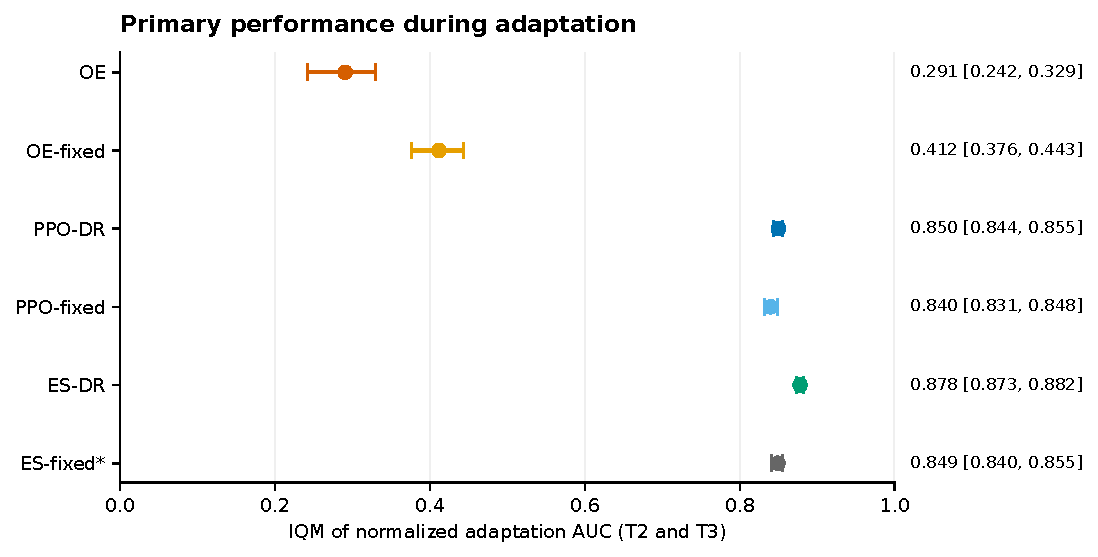
\includegraphics[width=0.92\linewidth]{figures/fig02_primary.pdf}
\caption{\textbf{Performance during adaptation on T2 and T3.} Points show pooled IQMs of normalized AUC; bars are nominal 95\% whole-run percentile bootstrap intervals from 50,000 draws. Each procedure has ten training runs evaluated on twenty fixed environments. Asterisk: ES-fixed was added after the core experiment.}
\label{fig:primary}
\end{figure}

OE is already below PPO-DR before adaptation. The zero-shot IQM difference on T2/T3 is $-0.4648$; at the final checkpoint it is $-0.6035$ (S4 and S5, both Holm-adjusted $p=0.00110$). Figure~\ref{fig:curves} shows the mean trajectories. In T2, OE's mean normalized competence declines from $0.4383$ to $0.2338$, while PPO-DR changes from $0.7244$ to $0.7478$. T3 shows a smaller decline for OE, from $0.2966$ to $0.2655$.

On the in-range T1 suite, the OE--PPO-DR difference in adaptation AUC is $-0.5371$ (nominal 95\% interval $[-0.5951,-0.4799]$; S6). 

\subsection{Fixed and varied training}
The separately tuned varied OE procedure scores below OE-fixed on T2/T3 AUC: difference $-0.1210$, interval $[-0.1799,-0.0680]$ (S2; Holm-adjusted $p=0.00440$). For PPO, the corresponding difference is $0.0099$, interval $[-0.0004,0.0201]$. Its predicted direction is unsupported under the prespecified rank-test rule (S3; adjusted $p=0.6232$).

In the later ES-fixed extension, ES-DR has higher T2/T3 adaptation AUC by $0.0286$ (nominal 95\% interval $[0.0203,0.0384]$), below the $0.05$ margin. The corresponding rank test gives adjusted $p=0.000365$. ES-DR also has higher T1 zero-shot competence by $0.0645$ (interval $[0.0499,0.0788]$; adjusted $p=0.000365$).

Selected hyperparameters also differ between fixed and varied configurations. For OE, the mutation standard deviation is $0.03412$ under varied training and $0.00507$ under fixed training.

\begin{figure}[tb]
\centering
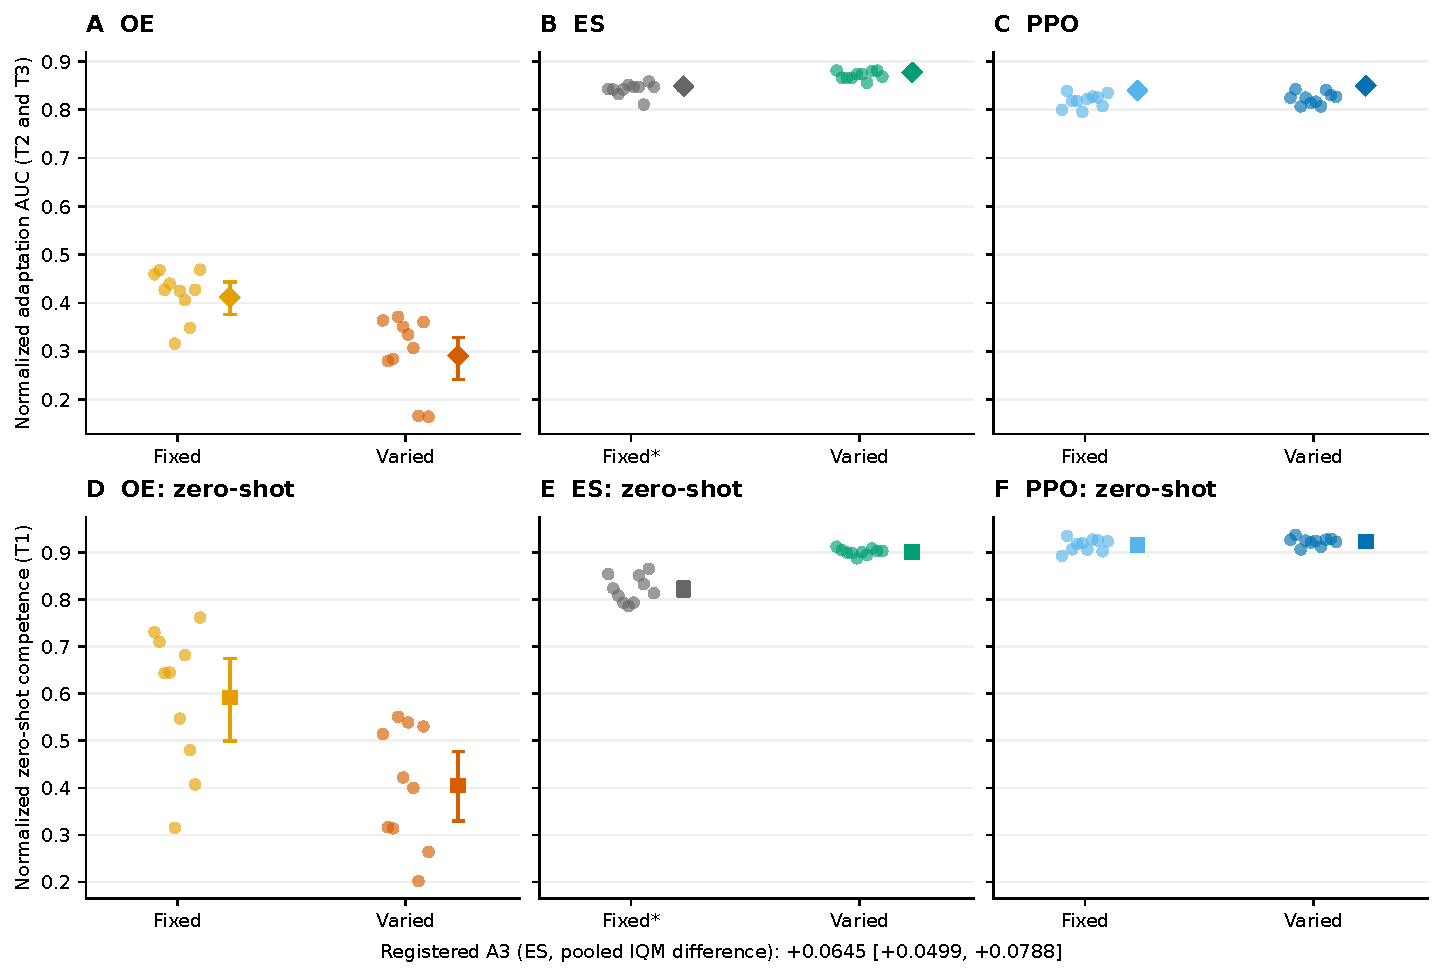
\includegraphics[width=\linewidth]{figures/fig03_variation.pdf}
\caption{\textbf{Fixed and varied configurations.} Upper panels: T2/T3 AUC, with run means (circles), pooled IQMs (diamonds) and nominal 95\% whole-run intervals. Lower panels: T1 zero-shot run means and their mean (squares), with descriptive 95\% intervals from 20,000 whole-run bootstrap draws. A3 denotes the pooled-IQM contrast; lower OE/PPO panels are descriptive. Each configuration was tuned separately. Asterisk: ES-fixed extension.}
\label{fig:variation}
\end{figure}

\subsection{Population persistence and support}
OE has higher extinction in the separate persistence assay than PPO-DR. Across T2/T3, the S7 difference in IQMs of per-run extinction fractions is $0.3750$, interval $[0.2500,0.4833]$, against the predicted OE advantage (adjusted $p=0.00110$). Table~\ref{tab:persistence} reports the descriptive extinction frequencies for every procedure. Extinction is frequent across all six procedures in resource-scarce T2, including those with high normalized competence. High relative food acquisition can coexist with insufficient intake for population survival.

\begin{table}[tb]
\centering\small
\caption{Descriptive extinction frequencies in the separate 5,000-step no-floor assay. Each cell pools ten runs across ten fixed environments; these 100 observations are not independent training runs.}\label{tab:persistence}
\begin{tabularx}{\linewidth}{lYYY}
\toprule
Procedure & T1 & T2 & T3\\\midrule
OE & 0.48 & 0.94 & 0.76\\
OE-fixed & 0.30 & 0.93 & 0.48\\
PPO-DR & 0.03 & 0.83 & 0.15\\
PPO-fixed & 0.10 & 0.95 & 0.14\\
ES-DR & 0.03 & 0.89 & 0.22\\
ES-fixed* & 0.11 & 0.87 & 0.21\\
\bottomrule
\end{tabularx}
\end{table}


The population floor makes a substantial contribution during OE training and adaptation. The mean run-level share of training births supplied by the floor is approximately $58\%$ for OE and $59\%$ for OE-fixed. During T2 adaptation, the pooled shares rise to $99.53\%$ and $99.60\%$, respectively (Table~\ref{tab:floor}).

\begin{table}[tb]
\centering\small
\caption{Share of new agents supplied by population-floor replacements during adaptation. Fractions pool event counts over ten runs and ten environments per suite.}\label{tab:floor}
\begin{tabularx}{\linewidth}{lYY}
\toprule
Suite & OE & OE-fixed\\\midrule
T1 & 64.35\% & 59.29\%\\
T2 & 99.53\% & 99.60\%\\
T3 & 78.90\% & 71.87\%\\
\bottomrule
\end{tabularx}
\end{table}


\subsection{Learning curves}
Between the first validation checkpoint near 20 million steps and the end of training at 200 million steps, OE's mean score above random increases from $9.4818$ to $10.6102$; six of ten runs improve (Figure~\ref{fig:curves}). Three additional exploratory runs extend OE training to one billion steps (Appendix~\ref{app:diagnostics}).

\begin{figure}[!t]
\centering
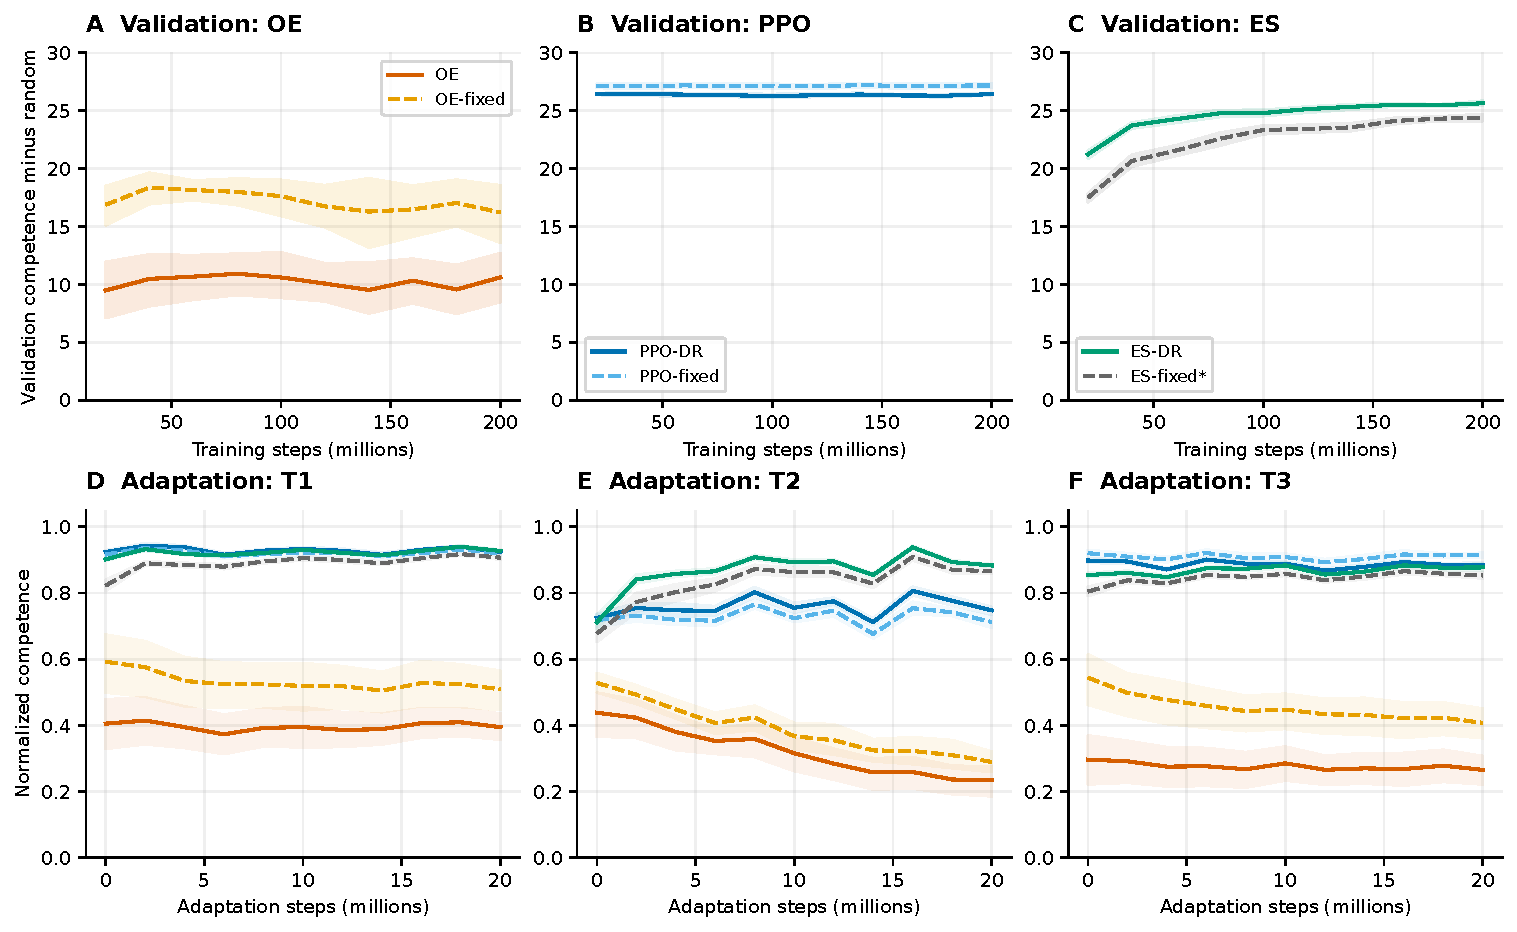
\includegraphics[width=\linewidth]{figures/fig04_curves.pdf}
\caption{\textbf{Training and adaptation.} Upper panels: validation competence above the random reference. Lower panels: normalized test competence during adaptation. Lines average ten runs; shading gives pointwise 95\% whole-run percentile intervals from 20,000 draws. Axes use nominal living-agent steps. Training measurements begin near 20 million steps.}
\label{fig:curves}
\end{figure}

The OE--PPO-DR contrast remains negative under paired-seed resampling, re-estimation of normalization anchors and integration over actual step counts. The weaker PPO fixed/varied comparison depends on the summary and resampling method (Appendix~\ref{app:diagnostics}).

\FloatBarrier
\section{Discussion}
OE scores below PPO-DR before and during adaptation, and its populations have poorer persistence without floor support. The methods differ in several respects: OE selects an interacting population through survival and reproduction, whereas ES and PPO optimize episodic food acquisition and deploy copies of one actor. Separate tuning adds differences in hyperparameters. The experiment compares these configurations without isolating the contribution of each component.

Varied training has different outcomes across methods. The positive ES zero-shot contrast on T1 agrees in direction with \citet{milano2019moderate}; its adaptation contrast on the shifted suites is smaller. Varied OE scores below OE-fixed. We did not sweep the rate of environmental change, so the comparison does not test the moderate-rate optimum found in their study.

In resource-scarce T2, even policies with high normalized food scores frequently go extinct. Relative food acquisition and population survival measure different outcomes: survival requires enough intake to cover energy costs. Floor replacements supply additional energy during OE training and adaptation and account for over 99\% of births in T2. This dependence makes the population floor a central part of the tested OE procedure.

The results cover one foraging world and thirty fixed test environments. Tests in other environments and comparisons with matched hyperparameters, objectives and population structure would help determine which aspects of the procedures account for the observed differences.

\section{Conclusion}
In this foraging task, ecological neuroevolution performs below PPO-DR during adaptation and has poorer persistence without replacement support. Varied training scores below fixed training for OE, slightly above it for ES, and gives no supported advantage for PPO under the prespecified test.

\section*{Data and code availability}
Code, data and manuscript source are available at \url{https://github.com/Guntikiwritescode/ecological-neuroevolution}. Reproduction instructions are in \texttt{REPRODUCE.md}.

\section*{Author contributions}
Abhinav Guntaka designed the study, implemented the software, ran the experiments, analyzed the results and wrote the manuscript.

\section*{Funding and competing interests}
The author funded this work at a total cost of US\$87 and declares no competing interests.

\section*{Acknowledgements}
Claude Code, Cursor Agents and ChatGPT/Codex assisted with coding, analysis and manuscript preparation.

\bibliographystyle{plainnat}
\bibliography{references}
\clearpage
\appendix
\section{Implementation and selected settings}
\label{app:implementation}
The actor has dimensions $30\rightarrow32\rightarrow32\rightarrow2$, with tanh hidden activations and 2,114 parameters. Initial weights are orthogonal, with gain $\sqrt{2}$ in hidden layers and $0.01$ in the action layer; biases start at zero. The world maps the outputs through tanh to a turn bounded by $\pi/4$ per step and a speed between zero and the body's maximum. Evaluation actions are deterministic. The observation includes clipped energy divided by birth energy and scaled body traits, even though the latter remain fixed.

The per-step energy cost is $0.5+s^3v^2+0.05r$, where $s$ is size, $v$ is commanded speed after action squashing but before position clipping at a wall, and $r$ is sensing range. With the default body it is $1+v^2$. Food supplies 40 energy units. Ecological reproduction requires energy at least 200, costs the parent 120 and supplies the offspring with 100. Maximum age is 1,000 steps and the offspring placement offset is 1. The ecological capacity is 128; competence evaluation has 16 agent slots. The floor rule described in Section~\ref{sec:procedures} adds energy from outside this budget and is logged separately.

Within a step, agents move, consume reachable food, pay costs, die and reproduce; food dynamics then update. Random priority resolves contested food. Births require free slots, with eligible parents processed in random order, at most one child per parent per step, and payment only for successful births. At a varied-OE environment change, positions are clipped to the new arena as needed, while energy, age and genomes persist. Food is reinitialized under the new parameters.

For PPO, the common settings are 64 parallel worlds, 32 minibatches, GAE parameter 0.95, clipping parameter 0.2, value-loss coefficient 0.5, maximum gradient norm 0.5, initial log standard deviation zero and no learning-rate annealing. The separately selected values are in Table~\ref{tab:settings}. PPO's actor parameters, critic parameters, log standard deviation and reward-normalization state are carried into adaptation; its return accumulator, optimizer, environment state, counters and random stream are reset. OE carries controller genomes and the alive mask, while resetting positions, headings, energy, age, actions and counters. ES carries its mean solution while restarting its optimizer/strategy and generation counter.

The PPO critic has the same two hidden layers as the actor and a scalar output. Action exploration is Gaussian with learned, state-independent log standard deviation. The adapted implementation starts from PureJaxRL commit \texttt{31756b1}; ES uses evosax version 0.3.2. Source notices and licenses are retained with the scientific implementation.

\Needspace{14\baselineskip}
{\small
\begin{longtable}{lP{12cm}}
\caption{Selected hyperparameters, rounded to six significant digits. Exact values are in the accompanying tuning CSV. Asterisk: ES-fixed extension.}\label{tab:settings}\\
\toprule
Procedure & Settings\\\midrule
\endfirsthead
\toprule
Procedure & Settings\\\midrule
\endhead
\bottomrule\endfoot
OE & Mutation SD = 0.0341186\\
OE-fixed & Mutation SD = 0.00507475\\
PPO-DR & Entropy coefficient = 0; Discount = 0.99; Learning rate = 0.000180353; Reward normalization = on; Rollout length = 64; Update epochs = 8\\
PPO-fixed & Entropy coefficient = 0; Discount = 0.95; Learning rate = 0.000706297; Reward normalization = off; Rollout length = 128; Update epochs = 8\\
ES-DR & Episodes per candidate = 1; Learning rate = 0.0073746; Population size = 64; Perturbation SD = 0.089879\\
ES-fixed* & Episodes per candidate = 4; Learning rate = 0.0117805; Population size = 32; Perturbation SD = 0.0441052\\
\end{longtable}
}


The tuning search for PPO sampled learning rate log-uniformly from $10^{-4}$ to $10^{-3}$, rollout length from $\{32,64,128\}$, update epochs from $\{2,4,8\}$, discount from $\{0.95,0.99,0.995\}$, entropy coefficient from $\{0,0.001,0.01\}$ and reward normalization on or off. ES sampled perturbation scale from $[0.01,0.1]$ and learning rate from $[0.003,0.03]$, both log-uniformly, population size from $\{32,64,128\}$ and episodes per candidate from $\{1,2,4\}$. OE sampled weight-mutation standard deviation log-uniformly from $[0.005,0.05]$. Population floor and change interval were design choices, not tuned parameters. Each trial had its own tuning seed; a score tie favored the lower trial index.

Validation environments used seeds 4900--4919 plus four corner cases. Final T1, T2 and T3 environments used seeds 5900--5909, 5910--5919 and 5920--5929. Competence episodes were keyed from environment-specific evaluation seeds and checkpoint indices; the same test conditions were used across methods. Final run seeds were 5000--5009. The implementation separates named random streams by purpose, although common seeds can still couple methods. The exact realized environment parameters, rather than only their generating ranges, are retained with every evaluation record.

\section{Complete neural comparisons}
\label{app:inference}
The original private protocol called H1 a prediction that OE would adapt faster than PPO-DR. Its specified statistic was the AUC in Equation~\ref{eq:auc}. AUC includes the starting score and measures performance during adaptation, not adaptation speed. H1 is against the prediction because its interval lies below $-0.05$. The analogous later A1 contrast is positive but wholly below $0.05$ (Table~\ref{tab:primaryrules}). The margin is a fraction of an empirical reference gap; it has no established interpretation outside this normalization scale.

The H1/A1 rule checks the interval in this order. An interval wholly above zero supports the predicted direction, qualified as below the margin if it also lies below $+0.05$. An interval wholly below zero is against that direction, qualified as below the margin if it also lies above $-0.05$. If neither condition holds, an interval contained in $[-0.05,+0.05]$ yields the protocol's no-meaningful-difference label; any other interval is inconclusive. Thus directional support is not the same as exceeding the practical margin. These labels inherit the interval-calibration limitations in Section~\ref{sec:statistics}.

\begin{table}[tb]
\centering\small
\caption{Interval-rule comparisons. A1 and A2 use the same ES contrast; they are not independent confirmations. The margin is 0.05 on the empirical normalized scale.}\label{tab:primaryrules}
\begin{tabularx}{\linewidth}{lYYY}
\toprule
ID & Comparison & Difference [interval] & Decision\\\midrule
H1 & OE minus PPO-DR & $-0.5592$ $[-0.6088,-0.5196]$ & Against predicted superiority\\
A1 & ES-DR minus ES-fixed & $+0.0286$ $[0.0203,0.0384]$ & Positive, below margin\\
\bottomrule
\end{tabularx}
\end{table}

\Needspace{14\baselineskip}
{\small
\begin{longtable}{lP{2.6cm}P{2.2cm}P{4.0cm}r}
\caption{Complete core S1--S7 and later A2--A3 families. Differences are pooled IQMs except S7, which uses IQMs of per-run extinction fractions. Intervals are nominal 95\% whole-run intervals. Holm correction is separate for the two families. The rank-test $p$ values apply to per-run summaries, not directly to the IQM effects.}\label{tab:tests}\\
\toprule
ID & Comparison & Outcome & Difference [interval] & Adjusted $p$\\\midrule
\endfirsthead
\toprule
ID & Comparison & Outcome & Difference [interval] & Adjusted $p$\\\midrule
\endhead
\bottomrule\endfoot
S1 & OE minus ES-DR & T2/T3 AUC & $-0.5871$ $[-0.6364,-0.5475]$ & 0.0011\\
S2 & OE minus OE-fixed & T2/T3 AUC & $-0.1210$ $[-0.1799,-0.0680]$ & 0.0044\\
S3 & PPO-DR minus PPO-fixed & T2/T3 AUC & $+0.0099$ $[-0.0004,0.0201]$ & 0.6232\\
S4 & OE minus PPO-DR & T2/T3 zero-shot & $-0.4648$ $[-0.5570,-0.4073]$ & 0.0011\\
S5 & OE minus PPO-DR & T2/T3 final & $-0.6035$ $[-0.6486,-0.5643]$ & 0.0011\\
S6 & OE minus PPO-DR & T1 AUC & $-0.5371$ $[-0.5951,-0.4799]$ & 0.0011\\
S7 & OE minus PPO-DR & T2/T3 extinction & $+0.3750$ $[0.2500,0.4833]$ & 0.0011\\
A2 & ES-DR minus ES-fixed* & T2/T3 AUC & $+0.0286$ $[0.0203,0.0384]$ & $3.65\times10^{-4}$\\
A3 & ES-DR minus ES-fixed* & T1 zero-shot & $+0.0645$ $[0.0499,0.0788]$ & $3.65\times10^{-4}$\\
\end{longtable}
}


S1, S2, S5 and S7 are against their predicted OE directions. S3 does not support its predicted PPO direction. S4 and S6 were nondirectional and favor PPO-DR. A2 and A3 support the predicted ES-DR direction under the separate addendum family. The Mann--Whitney probability summary is $U/(n_Xn_Y)$, with ties contributing one half; the test is not generally a test of arithmetic mean equality. S7 first reduces each run to its extinction fraction across T2/T3, then compares the distributions of those fractions. It does not treat individual environments as independent training replications.

For H2b, write $q_{ov},q_{of},q_{pv},q_{pf}$ for pooled AUC IQMs of OE, OE-fixed, PPO-DR and PPO-fixed. The prespecified summaries are
\begin{align}
 V&=\tfrac12[(q_{ov}-q_{of})+(q_{pv}-q_{pf})],\\
 M&=\tfrac12[(q_{ov}-q_{pv})+(q_{of}-q_{pf})],\\
 I&=(q_{ov}-q_{of})-(q_{pv}-q_{pf}),\qquad
 \Delta=|V|-|M|.
\end{align}
Table~\ref{tab:four} reports the estimates. The original rule labeled the negative $\Delta$ interval ``method matters more.'' That label describes these four configurations on this scale. Their interaction is nonzero, and tuning differs, so it is not a general or causal main-effect statement. Absolute-value contrasts are also unstable when a component is close to zero.

A4 compares the ES varied-minus-fixed contrast with the corresponding OE contrast. Its difference is $0.149628$, interval $[0.095763,0.209123]$. A4 is descriptive: the OE outcome was known before the ES-fixed extension. Its component intervals come from the four-method resampling routine and need not exactly equal the intervals from separate two-method routines.

\begin{table}[tb]
\centering\small
\caption{Four-method contrasts. H2b covers the core configurations; A4 adds ES-fixed after the OE comparison was known.}\label{tab:four}
\begin{tabularx}{\linewidth}{lP{4.5cm}rY}
\toprule
Analysis & Quantity & Estimate & Nominal 95\% interval\\\midrule
H2b & $\Delta=|V|-|M|$ & -0.438162 & [-0.474258, -0.405598]\\
H2b & $I$ & -0.130959 & [-0.190704, -0.076383]\\
H2b & $M$ & -0.493721 & [-0.524014, -0.467100]\\
H2b & $V$ & -0.055559 & [-0.085238, -0.028180]\\
A4 & $I$ & +0.149628 & [0.095763, 0.209123]\\
A4 & ES-DR minus ES-fixed & +0.028590 & [0.020276, 0.038461]\\
A4 & OE minus OE-fixed & -0.121038 & [-0.179733, -0.067839]\\
\bottomrule
\end{tabularx}
\end{table}

\Needspace{14\baselineskip}
{\small
\begin{longtable}{llrrr}
\caption{Mean normalized performance, averaging environments within runs and then runs. Asterisk: ES-fixed extension.}\label{tab:descriptives}\\
\toprule
Procedure & Suite & Zero-shot & Final & AUC\\\midrule
\endfirsthead
\toprule
Procedure & Suite & Zero-shot & Final & AUC\\\midrule
\endhead
\bottomrule\endfoot
OE & T1 & 0.4052 & 0.3946 & 0.3960\\
OE & T2 & 0.4383 & 0.2338 & 0.3205\\
OE & T3 & 0.2966 & 0.2655 & 0.2759\\
OE-fixed & T1 & 0.5923 & 0.5088 & 0.5303\\
OE-fixed & T2 & 0.5285 & 0.2897 & 0.3860\\
OE-fixed & T3 & 0.5441 & 0.4076 & 0.4510\\
PPO-DR & T1 & 0.9236 & 0.9235 & 0.9295\\
PPO-DR & T2 & 0.7244 & 0.7478 & 0.7611\\
PPO-DR & T3 & 0.8981 & 0.8840 & 0.8861\\
PPO-fixed & T1 & 0.9161 & 0.9196 & 0.9216\\
PPO-fixed & T2 & 0.7181 & 0.7123 & 0.7290\\
PPO-fixed & T3 & 0.9202 & 0.9147 & 0.9089\\
ES-DR & T1 & 0.9017 & 0.9270 & 0.9231\\
ES-DR & T2 & 0.7114 & 0.8833 & 0.8743\\
ES-DR & T3 & 0.8543 & 0.8772 & 0.8686\\
ES-fixed* & T1 & 0.8223 & 0.9067 & 0.8930\\
ES-fixed* & T2 & 0.6770 & 0.8656 & 0.8377\\
ES-fixed* & T3 & 0.8041 & 0.8530 & 0.8470\\
\end{longtable}
}


\section{Sensitivity analyses and descriptive diagnostics}
\label{app:diagnostics}
Post hoc re-estimation of the core maximum anchor inside each of 50,000 bootstrap draws gives intervals of $[-0.61045,-0.52146]$ for H1, $[-0.17997,-0.06776]$ for S2, $[0.02042,0.03851]$ for A1 and $[0.04965,0.07903]$ for A3. Paired resampling of corresponding seeds gives $[-0.61012,-0.51847]$, $[-0.18100,-0.06919]$ and $[0.02039,0.03964]$ for H1, S2 and A1. S3's paired IQM interval is positive, as reported in the main text. None of these analyses replaces a prespecified test or establishes exact coverage for a selected maximum.

Realized adaptation counts differ between methods. The mean final counts per environment are approximately 20,000,010 for either OE variant, 20,017,188 for PPO-DR, 20,039,595 for PPO-fixed, 20,144,256 for ES-DR and 20,288,091 for ES-fixed. ES-fixed can overshoot its first two-million-step checkpoint by 49.5\%; the largest checkpoint excess is 4.98\% of the complete adaptation budget, and the largest final excess is 4.49\%. Actual-step sensitivity integrates the piecewise-linear saved observations and truncates at 20 million steps. Scores between saved checkpoints are linearly interpolated.

The primary deficit persists when individual runs or environments are omitted and when raw scores replace normalized scores. Figure~\ref{fig:profiles} shows empirical performance profiles and pairwise run-mean probability summaries.

\begin{figure}[tb]
\centering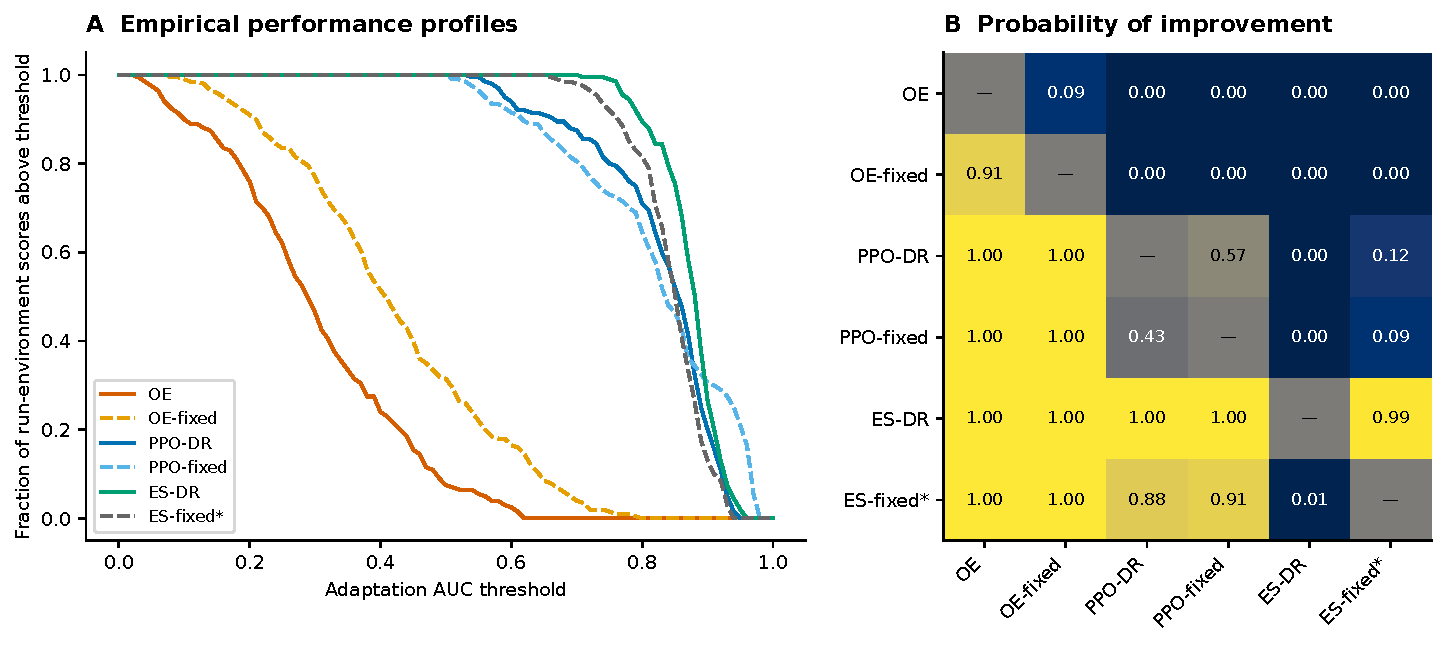
\includegraphics[width=\linewidth]{figures/fig05_profiles.pdf}
\caption{\textbf{Descriptive performance summaries.} Left: empirical fraction above each AUC threshold among ten runs across twenty fixed environments; no confidence bands are shown. Right: fraction of the 100 cross-run comparisons in which the row method's mean exceeds the column method's mean, with ties counting one half. These are descriptive effect summaries. ES-fixed is the later extension.}
\label{fig:profiles}
\end{figure}

The time-to-threshold diagnostic compares raw competence against 90\% of each run's mean T1 zero-shot score. It therefore depends on the food supply and attainable raw score in the target environment. In the core study, OE and OE-fixed each reach that threshold in 43 of 200 T2/T3 run--environment pairs; PPO-DR, PPO-fixed and ES-DR each reach it in 40. These counts are not independent trials and non-reaching cases cannot be dropped when interpreting adaptation. The threshold is not a general recovery criterion.

Population diversity is descriptive. Weight diversity is mean pairwise Euclidean distance among sixteen sampled neural parameter vectors. Behavior diversity uses action distances on 256 fixed validation probes. Body-trait diversity is zero by design. The final saved OE weight and behavior summaries exceed OE-fixed's, but no diversity intervention in this neural experiment identifies the effect of that difference (Figure~\ref{fig:diagnostics}).

\begin{figure}[p]
\centering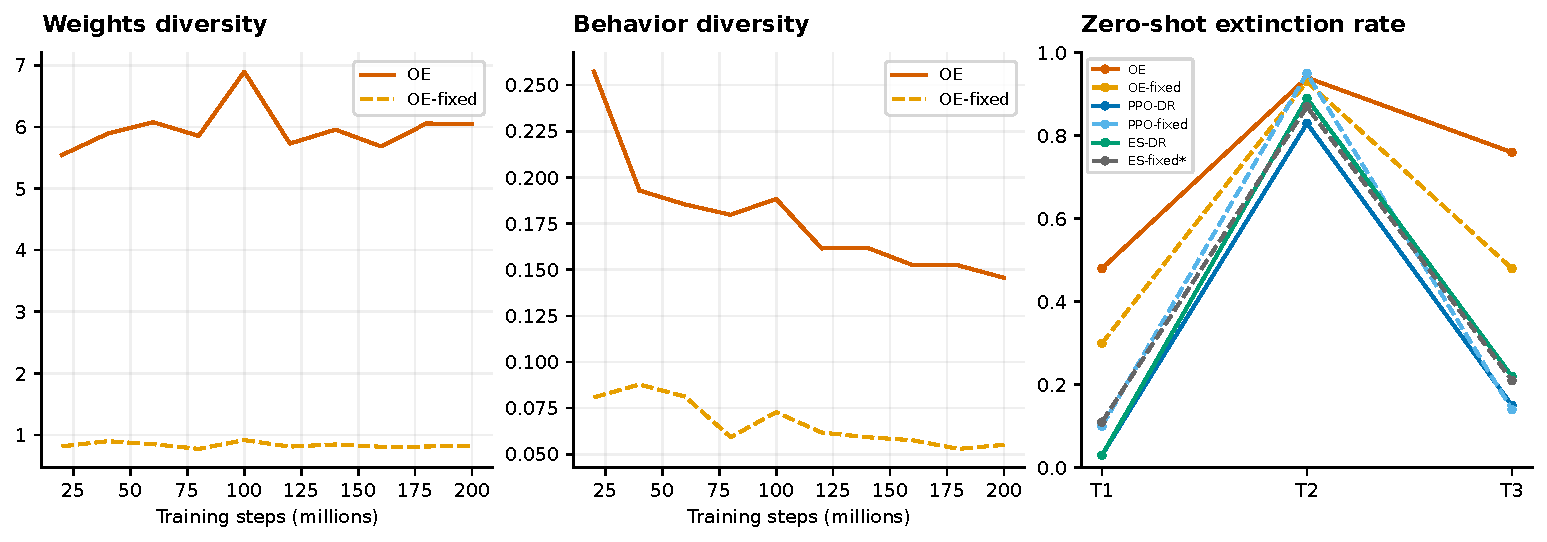
\includegraphics[width=\linewidth]{figures/figS01_diagnostics.pdf}
\caption{\textbf{Population diagnostics and separate persistence.} Weight and behavioral diversity summarize sixteen sampled agents per saved training population, averaged across ten runs. No uncertainty bands are assigned. The right panel shows extinction frequencies in the separate no-floor persistence assay, not extinction during floor-supported training. Body traits remain fixed.}
\label{fig:diagnostics}
\end{figure}

Three fresh OE runs were trained to one billion steps after the core results. Gain compares the final two saved validation checkpoints with the first two. None exceeded a prewritten 4.3-point threshold, whose motivating noise estimate was subsequently found unreliable; this is not a calibrated test. Figure~\ref{fig:long} shows their saved trajectories.

\begin{figure}[p]
\centering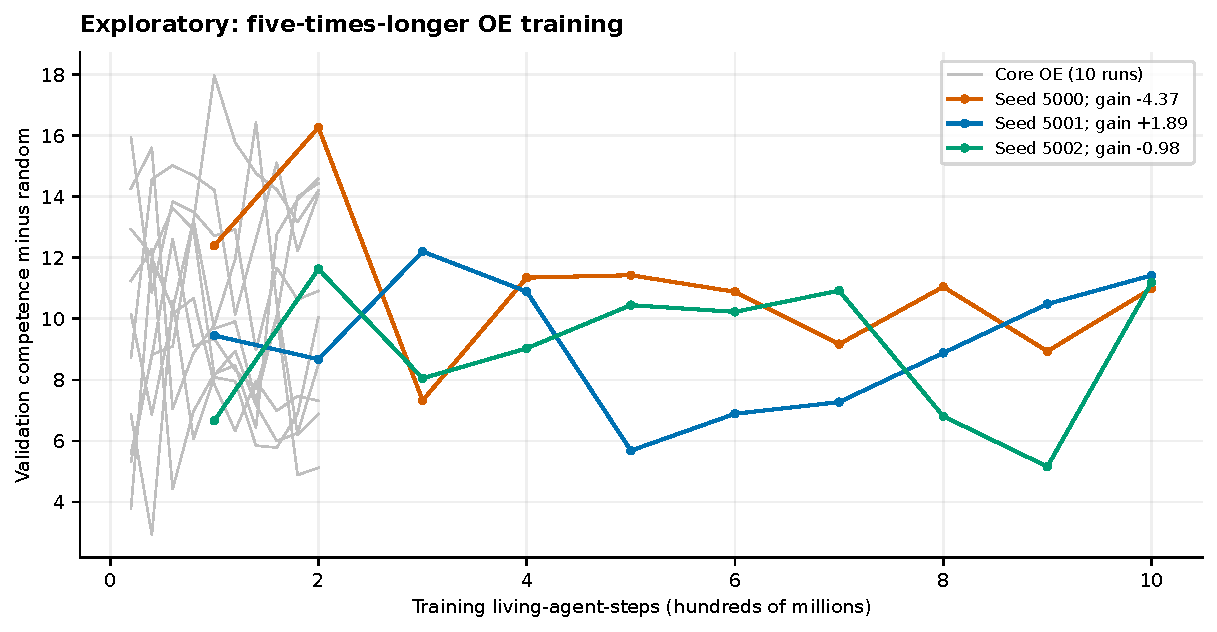
\includegraphics[width=0.9\linewidth]{figures/fig08_long_training.pdf}
\caption{\textbf{Exploratory longer training.} Three fresh OE runs trained to one billion nominal steps, with the ten original 200-million-step runs in gray. Gain is the mean of the final two saved checkpoints minus the mean of the first two. No inferential interval or significance test is assigned to these three runs. Same-seed trajectories need not agree across machines.}
\label{fig:long}
\end{figure}

\FloatBarrier
\section{Supporting trait-only experiment}
\label{app:trait}
\subsection{Design and analysis}
The trait model combines inherited speed, size, sensing range and reach with fixed behavioral rules. Populations spend 100 generations in environment A and 50 in B. Each final run seed defines its own searches and deployments. There are 200 seeds per primary group and arm (2000--2199). Shared food, behavior and initial-position streams couple groups with the same seed. The main B has 25 food items; three additional arms permit agent consumption in B, enlarge the B map to side 750, or reduce B's energy budget per generation to 25. The larger-map and reduced-energy settings were selected during recorded pilot and amendment rounds before the corresponding final runs.

The generation rules derive from the MinuteLabs Evolution Simulator at commit \texttt{55af956} \citep{palfree_evolution_simulator}. A has side length 500 and 50 uniformly placed food items. Main B has side length 300 and 25 items in five clusters with standard deviation 15; centers and food are redrawn each generation. A generation lasts at most 200 ticks, with an energy allowance of 500 per agent except in the reduced-energy B arm. Agents start at edge home positions, search using fixed steering rules and return home according to feeding and remaining energy. Exhaustion and, in the consumption arm, predation can kill agents; agents with no food at generation end also die. Survivors carry into the next generation, and each survivor that consumed at least two food units produces exactly one offspring. Food units count both food items and prey. Effective movement speed is $u=\text{speed}\times\text{size}/10$, and each active movement tick costs $10^{-4}(\text{size}^3u^2+\text{sense})$. Food supports survival and reproduction without replenishing this generation-level energy allowance. There is no externally supported population floor.

Initial populations have 50 agents. ET starts from speed/size/sense/reach values $10/10/20/1$. Mutating offspring receive independent Gaussian trait perturbations with standard deviations $1/1/1/0.25$; sensing range is clipped at zero and the other traits at the smallest positive normalized float64 value. ET and M-pop mutate in both phases. F-food, F-pop, SV and Oracle-B have mutation disabled throughout. ET-freeze and ET-clone are derived from ET after A and have mutation disabled in B. SV samples each trait independently and log-uniformly over the search ranges: speed and size 2.5--40, sense 5--80 and raw reach 0.25--4.

In the consumption arm, a predator can consume only an agent whose size is at most 80\% of its own. Identical clones therefore cannot consume one another. Comparisons involving clones and heterogeneous populations also differ in access to this additional food source; differences among heterogeneous groups depend on their size distributions. Across all 50 B generations, mean prey counts per run are 150.8 for ET, 153.2 for M-pop, 18.4 for ET-freeze and 3.4 for SV, with zero for the four homogeneous frozen groups.

The A search begins with eight logarithmically spaced values for each trait. Merging designs with the same effective reach, $\max(\text{reach},\text{size}/4)$, leaves 1,472 distinct designs. Stage one evaluates 50 clones of each design for 30 generations on shared streams. Stage two evaluates the top 32 designs per objective on eight fresh sets of streams. Population search scores mean population over generations 10--99; food search scores food per agent over generations 10--29, even when a candidate was simulated for longer. The comparison therefore changes both objective and scoring horizon. Search-selected mutating agents inherit effective reach.

The group identifiers used in the tables are: ET, the evolving population; F-food and F-pop, frozen copies of the food- and population-search winners; M-pop, mutating copies of the population-search winner; SV, a frozen initial population with standing variation; ET-freeze, the end-of-A evolved population with mutation disabled in B; ET-clone, copies of a randomly sampled end-of-A member with mutation disabled; and Oracle-B, the reference design selected directly in B. Oracle-B is not part of the confirmatory contrast family. Cloning changes the realized traits along with heterogeneity.

P1 is population at the start of a generation, averaged over B generations 40--49 with zeros retained. P2 indicates that no agent would start B generation 50. Each arm has eight planned comparison pairs, except arm 2 omits the population-search versus food-search pair because those data repeat the main arm by construction: 31 pairs in total. P1 uses a two-sided 10,000-permutation test of mean differences and a studentized bootstrap interval with 20,000 draws. P2 uses a two-sided Fisher test and a Newcombe interval for the difference in extinction proportions. Holm adjustment is within each arm's 16-test family, or 14 tests for arm 2. Shared streams make independent-group test calibration an approximation; paired sensitivity is retained separately in the supporting analysis records.

The practical margins are 2.5 agents for P1 and 0.10 for P2. The original ``meaningfully different'' label requires adjusted $p<0.05$ and an absolute point estimate at least as large as the margin; it does not require the entire interval to exceed it. Equivalence uses an interval at level $1-2(0.05)/k$, where $k$ is the arm's family size, wholly inside the margins. These equivalence intervals are wider than the 95\% intervals printed below. Boundary labels distinguish ceiling, one-sided ceiling and floor cases. Equivalence near a population ceiling does not establish interchangeable adaptability.

\subsection{Full primary outcome family and diagnostic controls}
Table~\ref{tab:traitcontrasts} reports all 31 pairs and both outcomes. Table~\ref{tab:traitgroups} gives every primary group's mean population, extinction count, pre-shift losses and boundary frequencies. Full text labels, including ceiling qualifications and A-phase-loss flags, are also retained in \texttt{data/trait\_complete\_contrasts.csv}. Figure~\ref{fig:trait} provides the group-level display; its intervals do not replace the contrast rules.

\begin{figure}[tb]
\centering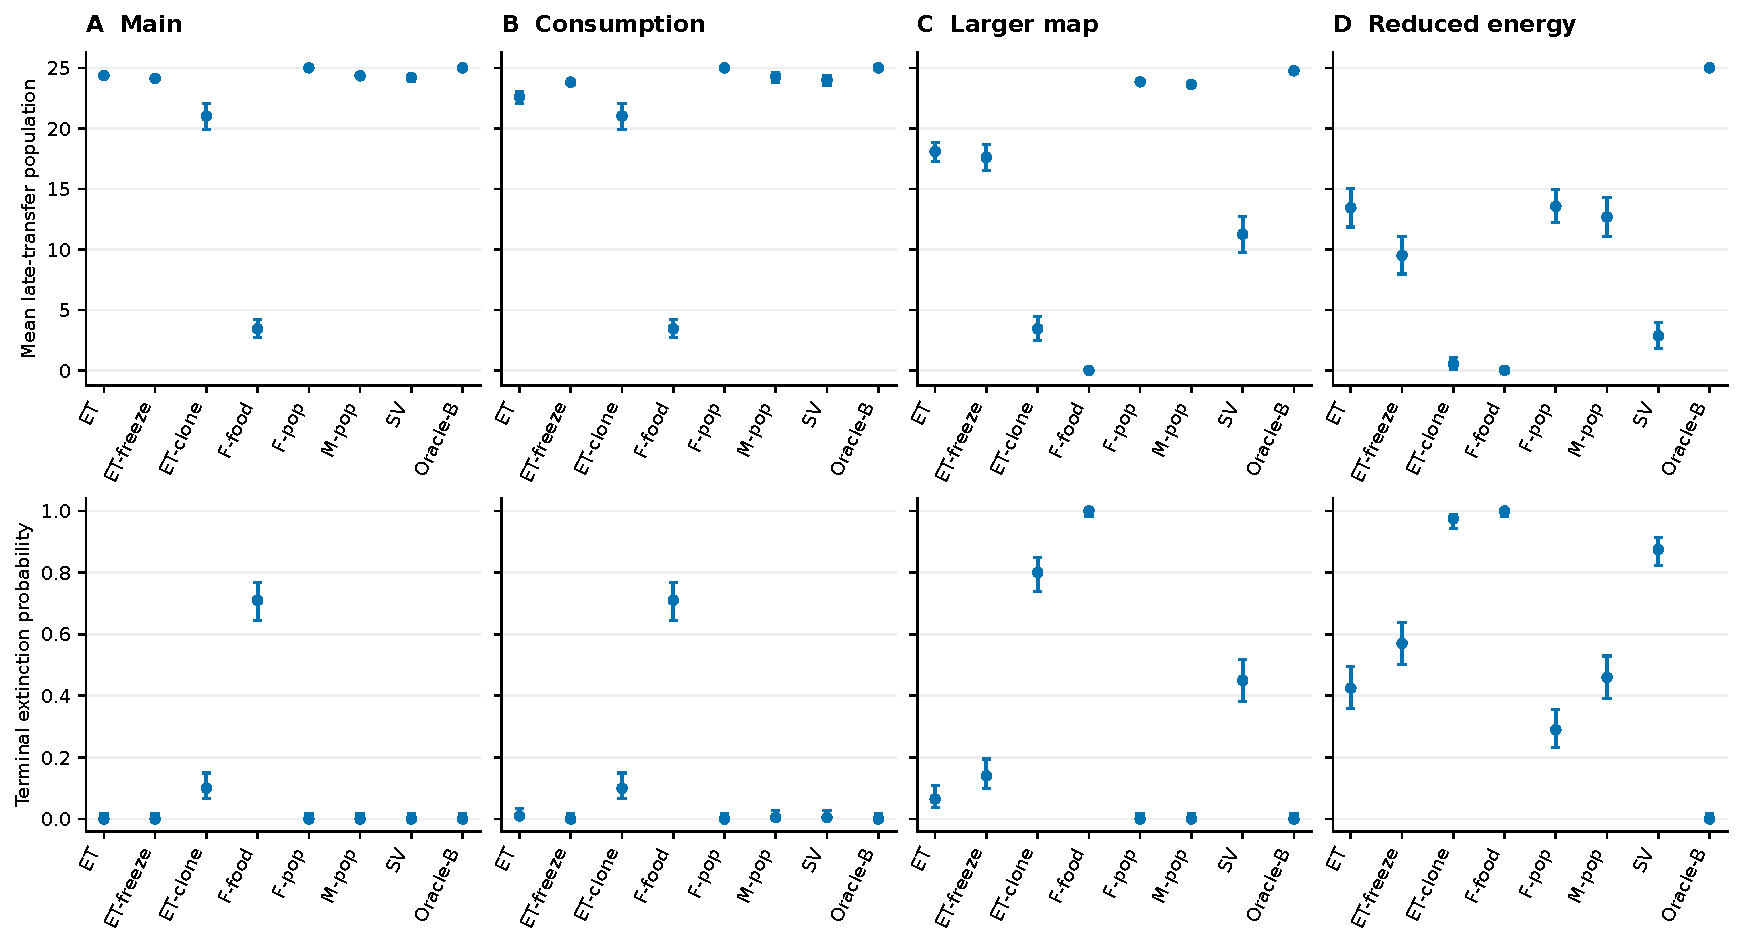
\includegraphics[width=\linewidth]{figures/fig07_trait_experiment.pdf}
\caption{\textbf{Supporting trait experiment.} All eight primary groups in four arms, with 200 seeds per group. Upper panels: mean P1 and descriptive whole-seed percentile 95\% intervals (20,000 draws). Lower panels: P2 proportions with Wilson 95\% intervals. These differ from the studentized P1 and Newcombe P2 intervals for contrasts. Shared seeds induce dependence across groups. Population and food searches differ in objective and scoring horizon; no-shift controls constrain diversity interpretations.}
\label{fig:trait}
\end{figure}

\Needspace{14\baselineskip}
{\small
\begin{longtable}{lP{2.7cm}P{3cm}P{2.8cm}P{2.5cm}l}
\caption{All 31 trait-study comparison pairs; all differences are X minus Y, with comparisons written X / Y. P1 is mean late-B population and P2 is terminal extinction probability. Entries are differences with 95\% intervals. MD: significant with point estimate at or beyond the margin; EQ: equivalence under the specified interval rule; DU: detected difference with size unresolved; IN: inconclusive. Boundary qualifications are in Table~\ref{tab:traitgroups}; full labels are retained in the accompanying CSV.}\label{tab:traitcontrasts}\\
\toprule
Arm-row & X / Y & P1 difference [CI] & P2 difference [CI] & Adj. $p_1$ / $p_2$ & P1/P2\\\midrule
\endfirsthead
\toprule
Arm-row & X / Y & P1 difference [CI] & P2 difference [CI] & Adj. $p_1$ / $p_2$ & P1/P2\\\midrule
\endhead
\bottomrule\endfoot
main-1 & F-food / ET & $-20.93$ $[-21.66,-20.11]$ & $+0.71$ $[0.64,0.77]$ & 0.0013 / $9.54\times10^{-60}$ & MD/MD\\
main-2 & F-pop / ET & $+0.64$ $[0.59,0.68]$ & $+0.00$ $[-0.02,0.02]$ & 0.0013 / 1 & EQ/EQ\\
main-3 & M-pop / ET & $-0.02$ $[-0.08,0.04]$ & $+0.00$ $[-0.02,0.02]$ & 1 / 1 & EQ/EQ\\
main-4 & SV / ET & $-0.16$ $[-0.64,0.10]$ & $+0.00$ $[-0.02,0.02]$ & 1 / 1 & EQ/EQ\\
main-5 & ET-freeze / ET & $-0.23$ $[-0.41,-0.08]$ & $+0.00$ $[-0.02,0.02]$ & 0.04 / 1 & EQ/EQ\\
main-6 & ET-clone / ET-freeze & $-3.11$ $[-4.36,-2.11]$ & $+0.10$ $[0.06,0.15]$ & 0.0013 / $1.62\times10^{-5}$ & MD/MD\\
main-7 & F-pop / F-food & $+21.57$ $[20.76,22.28]$ & $-0.71$ $[-0.77,-0.64]$ & 0.0013 / $9.54\times10^{-60}$ & MD/MD\\
main-8 & M-pop / F-pop & $-0.66$ $[-0.70,-0.62]$ & $+0.00$ $[-0.02,0.02]$ & 0.0013 / 1 & EQ/EQ\\
A2-1 & F-food / ET & $-19.16$ $[-20.02,-18.17]$ & $+0.70$ $[0.63,0.76]$ & 0.0012 / $5.18\times10^{-56}$ & MD/MD\\
A2-2 & F-pop / ET & $+2.41$ $[1.97,3.02]$ & $-0.01$ $[-0.04,0.01]$ & 0.0012 / 1 & DU/EQ\\
A2-3 & M-pop / ET & $+1.68$ $[1.05,2.34]$ & $-0.01$ $[-0.03,0.02]$ & 0.0012 / 1 & DU/EQ\\
A2-4 & SV / ET & $+1.40$ $[0.75,2.05]$ & $-0.01$ $[-0.03,0.02]$ & 0.0012 / 1 & EQ/EQ\\
A2-5 & ET-freeze / ET & $+1.24$ $[0.76,1.84]$ & $-0.01$ $[-0.04,0.01]$ & 0.0012 / 1 & EQ/EQ\\
A2-6 & ET-clone / ET-freeze & $-2.80$ $[-4.03,-1.81]$ & $+0.10$ $[0.06,0.15]$ & 0.0012 / $1.50\times10^{-5}$ & MD/MD\\
A2-8 & M-pop / F-pop & $-0.73$ $[-1.26,-0.38]$ & $+0.01$ $[-0.01,0.03]$ & 0.0018 / 1 & EQ/EQ\\
A3-1 & F-food / ET & $-18.10$ $[-18.83,-17.18]$ & $+0.94$ $[0.89,0.96]$ & 0.0012 / $5.98\times10^{-98}$ & MD/MD\\
A3-2 & F-pop / ET & $+5.74$ $[5.00,6.66]$ & $-0.07$ $[-0.11,-0.03]$ & 0.0012 / 0.0012 & MD/DU\\
A3-3 & M-pop / ET & $+5.53$ $[4.80,6.43]$ & $-0.07$ $[-0.11,-0.03]$ & 0.0012 / 0.0012 & MD/DU\\
A3-4 & SV / ET & $-6.86$ $[-8.56,-5.13]$ & $+0.39$ $[0.31,0.46]$ & 0.0012 / $1.48\times10^{-18}$ & MD/MD\\
A3-5 & ET-freeze / ET & $-0.50$ $[-1.87,0.81]$ & $+0.07$ $[0.02,0.14]$ & 0.9333 / 0.07 & EQ/IN\\
A3-6 & ET-clone / ET-freeze & $-14.16$ $[-15.54,-12.58]$ & $+0.66$ $[0.58,0.72]$ & 0.0012 / $1.44\times10^{-41}$ & MD/MD\\
A3-7 & F-pop / F-food & $+23.84$ $[23.70,23.97]$ & $-1.00$ $[-1.00,-0.97]$ & 0.0012 / $3.11\times10^{-118}$ & MD/MD\\
A3-8 & M-pop / F-pop & $-0.22$ $[-0.39,-0.04]$ & $+0.00$ $[-0.02,0.02]$ & 0.07 / 1 & EQ/EQ\\
A4-1 & F-food / ET & $-13.43$ $[-15.02,-11.81]$ & $+0.57$ $[0.50,0.64]$ & 0.0012 / $3.99\times10^{-44}$ & MD/MD\\
A4-2 & F-pop / ET & $+0.12$ $[-1.98,2.27]$ & $-0.14$ $[-0.23,-0.04]$ & 1 / 0.0329 & IN/MD\\
A4-3 & M-pop / ET & $-0.76$ $[-3.04,1.49]$ & $+0.04$ $[-0.06,0.13]$ & 1 / 1 & IN/IN\\
A4-4 & SV / ET & $-10.58$ $[-12.43,-8.63]$ & $+0.45$ $[0.36,0.53]$ & 0.0012 / $1.01\times10^{-20}$ & MD/MD\\
A4-5 & ET-freeze / ET & $-3.93$ $[-6.12,-1.66]$ & $+0.14$ $[0.05,0.24]$ & 0.0032 / 0.0303 & MD/MD\\
A4-6 & ET-clone / ET-freeze & $-8.97$ $[-10.63,-7.33]$ & $+0.41$ $[0.33,0.48]$ & 0.0012 / $1.39\times10^{-23}$ & MD/MD\\
A4-7 & F-pop / F-food & $+13.55$ $[12.15,14.93]$ & $-0.71$ $[-0.77,-0.64]$ & 0.0012 / $9.54\times10^{-60}$ & MD/MD\\
A4-8 & M-pop / F-pop & $-0.88$ $[-3.02,1.24]$ & $+0.17$ $[0.08,0.26]$ & 1 / 0.0044 & IN/MD\\
\end{longtable}
}

\Needspace{14\baselineskip}
{\small
\begin{longtable}{llrrrrr}
\caption{Trait-study group outcomes and boundary diagnostics. All groups have 200 seeds. High/low are fractions with P1 at least 22.5 / at most 2.5. In the consumption arm, 25 is not a hard population ceiling. A-dead identifies losses preceding the environmental shift.}\label{tab:traitgroups}\\
\toprule
Arm & Group & Mean P1 & Extinct & A-dead & High & Low\\\midrule
\endfirsthead
\toprule
Arm & Group & Mean P1 & Extinct & A-dead & High & Low\\\midrule
\endhead
\bottomrule\endfoot
Main & F-food & 3.43 & 142/200 & 62 & 0.00 & 0.69\\
Main & ET & 24.36 & 0/200 & 0 & 1.00 & 0.00\\
Main & F-pop & 25.00 & 0/200 & 0 & 1.00 & 0.00\\
Main & M-pop & 24.34 & 0/200 & 0 & 1.00 & 0.00\\
Main & SV & 24.20 & 0/200 & 0 & 0.92 & 0.00\\
Main & ET-freeze & 24.13 & 0/200 & 0 & 0.90 & 0.00\\
Main & ET-clone & 21.02 & 20/200 & 0 & 0.73 & 0.10\\
Main & Oracle-B & 25.00 & 0/200 & 0 & 1.00 & 0.00\\
Consumption & F-food & 3.43 & 142/200 & 62 & 0.00 & 0.69\\
Consumption & ET & 22.59 & 2/200 & 0 & 0.61 & 0.01\\
Consumption & F-pop & 25.00 & 0/200 & 0 & 1.00 & 0.00\\
Consumption & M-pop & 24.27 & 1/200 & 0 & 0.85 & 0.01\\
Consumption & SV & 23.99 & 1/200 & 0 & 0.90 & 0.01\\
Consumption & ET-freeze & 23.82 & 0/200 & 0 & 0.86 & 0.00\\
Consumption & ET-clone & 21.02 & 20/200 & 0 & 0.73 & 0.10\\
Consumption & Oracle-B & 25.00 & 0/200 & 0 & 1.00 & 0.00\\
Larger map & F-food & 0.00 & 200/200 & 62 & 0.00 & 1.00\\
Larger map & ET & 18.10 & 13/200 & 0 & 0.10 & 0.07\\
Larger map & F-pop & 23.84 & 0/200 & 0 & 0.93 & 0.00\\
Larger map & M-pop & 23.63 & 0/200 & 0 & 0.94 & 0.00\\
Larger map & SV & 11.24 & 90/200 & 0 & 0.24 & 0.45\\
Larger map & ET-freeze & 17.60 & 28/200 & 0 & 0.33 & 0.14\\
Larger map & ET-clone & 3.44 & 160/200 & 0 & 0.04 & 0.79\\
Larger map & Oracle-B & 24.76 & 0/200 & 0 & 1.00 & 0.00\\
Reduced energy & F-food & 0.00 & 200/200 & 62 & 0.00 & 1.00\\
Reduced energy & ET & 13.43 & 85/200 & 0 & 0.50 & 0.42\\
Reduced energy & F-pop & 13.55 & 58/200 & 0 & 0.34 & 0.28\\
Reduced energy & M-pop & 12.67 & 92/200 & 0 & 0.54 & 0.46\\
Reduced energy & SV & 2.85 & 175/200 & 0 & 0.09 & 0.88\\
Reduced energy & ET-freeze & 9.50 & 114/200 & 0 & 0.28 & 0.56\\
Reduced energy & ET-clone & 0.54 & 195/200 & 0 & 0.01 & 0.97\\
Reduced energy & Oracle-B & 25.00 & 0/200 & 0 & 1.00 & 0.00\\
\end{longtable}
}


In the main arm, the food-search group's deficit includes 62 of 200 runs lost during A. Restricting analysis to groups that both reach B selects survivors and can bias the comparison; such conditional outcomes are retained as diagnostics rather than replacing unconditional results. The no-move control continues ET's end-of-A population for fifty further generations in A. Mean late population is 48.0675 with mutation, 47.9895 after freezing, and 40.9730 after cloning. The freeze-minus-mutation difference is $-0.0780$, interval $[-0.2720,0.1140]$, which includes zero. The clone-minus-freeze difference is $-7.0165$, interval $[-9.1271,-5.0470]$. The clone deficit therefore also occurs without an environmental shift. No formal B-minus-A interaction test follows from comparing whether separate intervals include zero.

The predefined diagnostic that B might not require a different design is triggered in the main, consumption and larger-map arms, but not the reduced-energy arm. The positive control that B separates at least some groups holds in all four. The majority-single-design warning applies to the standing-variation group in all four arms. The search-reliability diagnostic U3 is not triggered. The U1 boundary frequencies and U4 pre-shift loss counts are shown in Table~\ref{tab:traitgroups}; they restrict how the apparent ties should be interpreted. No group exceeds the U4 threshold of losing more than half its runs during A.

Exploratory analyses use subsets of the retained seeds and do not change primary decisions. They cover alternative map sizes and food/tick settings, landscape ranks, half/double mutation sizes, longer B deployment, stage-one-only search winners, populations started directly in B, trait-change summaries, first-generation deaths, energy use and no-move controls. Their complete numerical outputs and sample sizes are preserved in \texttt{data/trait\_exploratory.json}. For example, on the 100-seed exploratory subset, starting ET directly in B instead of transferring from A changes P1 by $-0.22$ in the main arm, $-17.62$ in the larger-map arm and $-12.85$ in the reduced-energy arm. These initialization comparisons concern the trait model.

\clearpage
\section{Chronology and reproducibility}
\label{app:reproduction}
Pilot and tuning stages preceded the corresponding final runs. The private protocols specified five neural procedures and seven secondary comparisons. The pilot-based precision estimate used three seeds per method. Ten final runs were chosen per procedure, retaining the $0.05$ margin with limited precision for equivalence. ES-fixed was specified after inspection of the core results and before its own tuning and ten final runs. The one-billion-step OE extension was exploratory. Planned lifetime-learning and neural mechanism ablations were not run.

The neural core training and evaluation records identify revision \texttt{16e8657}; the ES-fixed extension identifies \texttt{06ff7b2}. Trait generation records identify \texttt{a1e1cdc} and the confirmatory analysis identifies \texttt{561bcd4}. The source inspection used revision \texttt{ea7792af7f66}. Full identifiers and configuration hashes are provided with the code.

Core neural records report NVIDIA RTX 4090 hardware, JAX 0.11.2 and Python 3.13.18. The statistical reanalysis used CPU execution with Python 3.12.14 and separately recorded dependencies. Two same-seed ES-DR check runs under the addendum configuration remained within the specified tolerance around the core range. Cross-machine runs need not be numerically identical. The test-access logs cover the recorded evaluations; access outside those logs cannot be assessed.

The archive contains all sixty final neural evaluations and 19,800 adaptation checkpoint observations, trait generation records, final trained policies, training snapshots and tuning-trial records. Core tuning policy files were not retained. A correction to detection of completely tied Mann--Whitney samples changed no reported effect, $p$ value or decision.

The repository includes source code, configurations, data, analysis scripts and the manuscript build files. Its README gives the commands for reproducing the tables, figures and statistical checks.

\end{document}
